%%%% File: rulers.tex
%%%% Provides 14-m worth of 1-m rulers at centimeter scale, all numbered, and
%%%% three 30-cm rulers, also numbered at every centimeter. 
%%%% Author: Ricardo Hernández, with much help from Qrrbrbirlbel
%%%% (http://tex.stackexchange.com/users/16595/qrrbrbirlbel) and the kind people
%%%% at TeX.Stackexchange. See: http://tex.stackexchange.com/a/121490/3731
%%%% Date: Saturday June 29, 2013
%%%% This file is meant to be printed three times, so as to have three sets of
%%%% 14-m rulers and 9 small 30-cm rulers. The rulers will be used on top and on
%%%% one side of a flume at the University of South Carolina, and on a bunch of
%%%% mounts placed atop the flume. It will be printed in low tack Photo Tex
%%%% paper. 


\documentclass[tikz,convert=false,12pt]{standalone}


%%%% Redefine the default font face to be sans serif, specifically a helvetica
%%%% clone called TeX Gyre Heros. 
\usepackage{tgheros}
\renewcommand*\familydefault{\sfdefault} 
\usepackage[T1]{fontenc}

%%%% Captures the last value of the \i iteration
\usepackage{calc}
\usepackage{pgffor}
\newcommand*{\lasti}{}



\begin{document}

%%%% Change the order of the TikZ coordinate system so that the rulers go from
%%%% right to left, at centimeter scale. Any unit not specified is multiplied by
%%%% -1 cm. This allows some fancy scaling. 
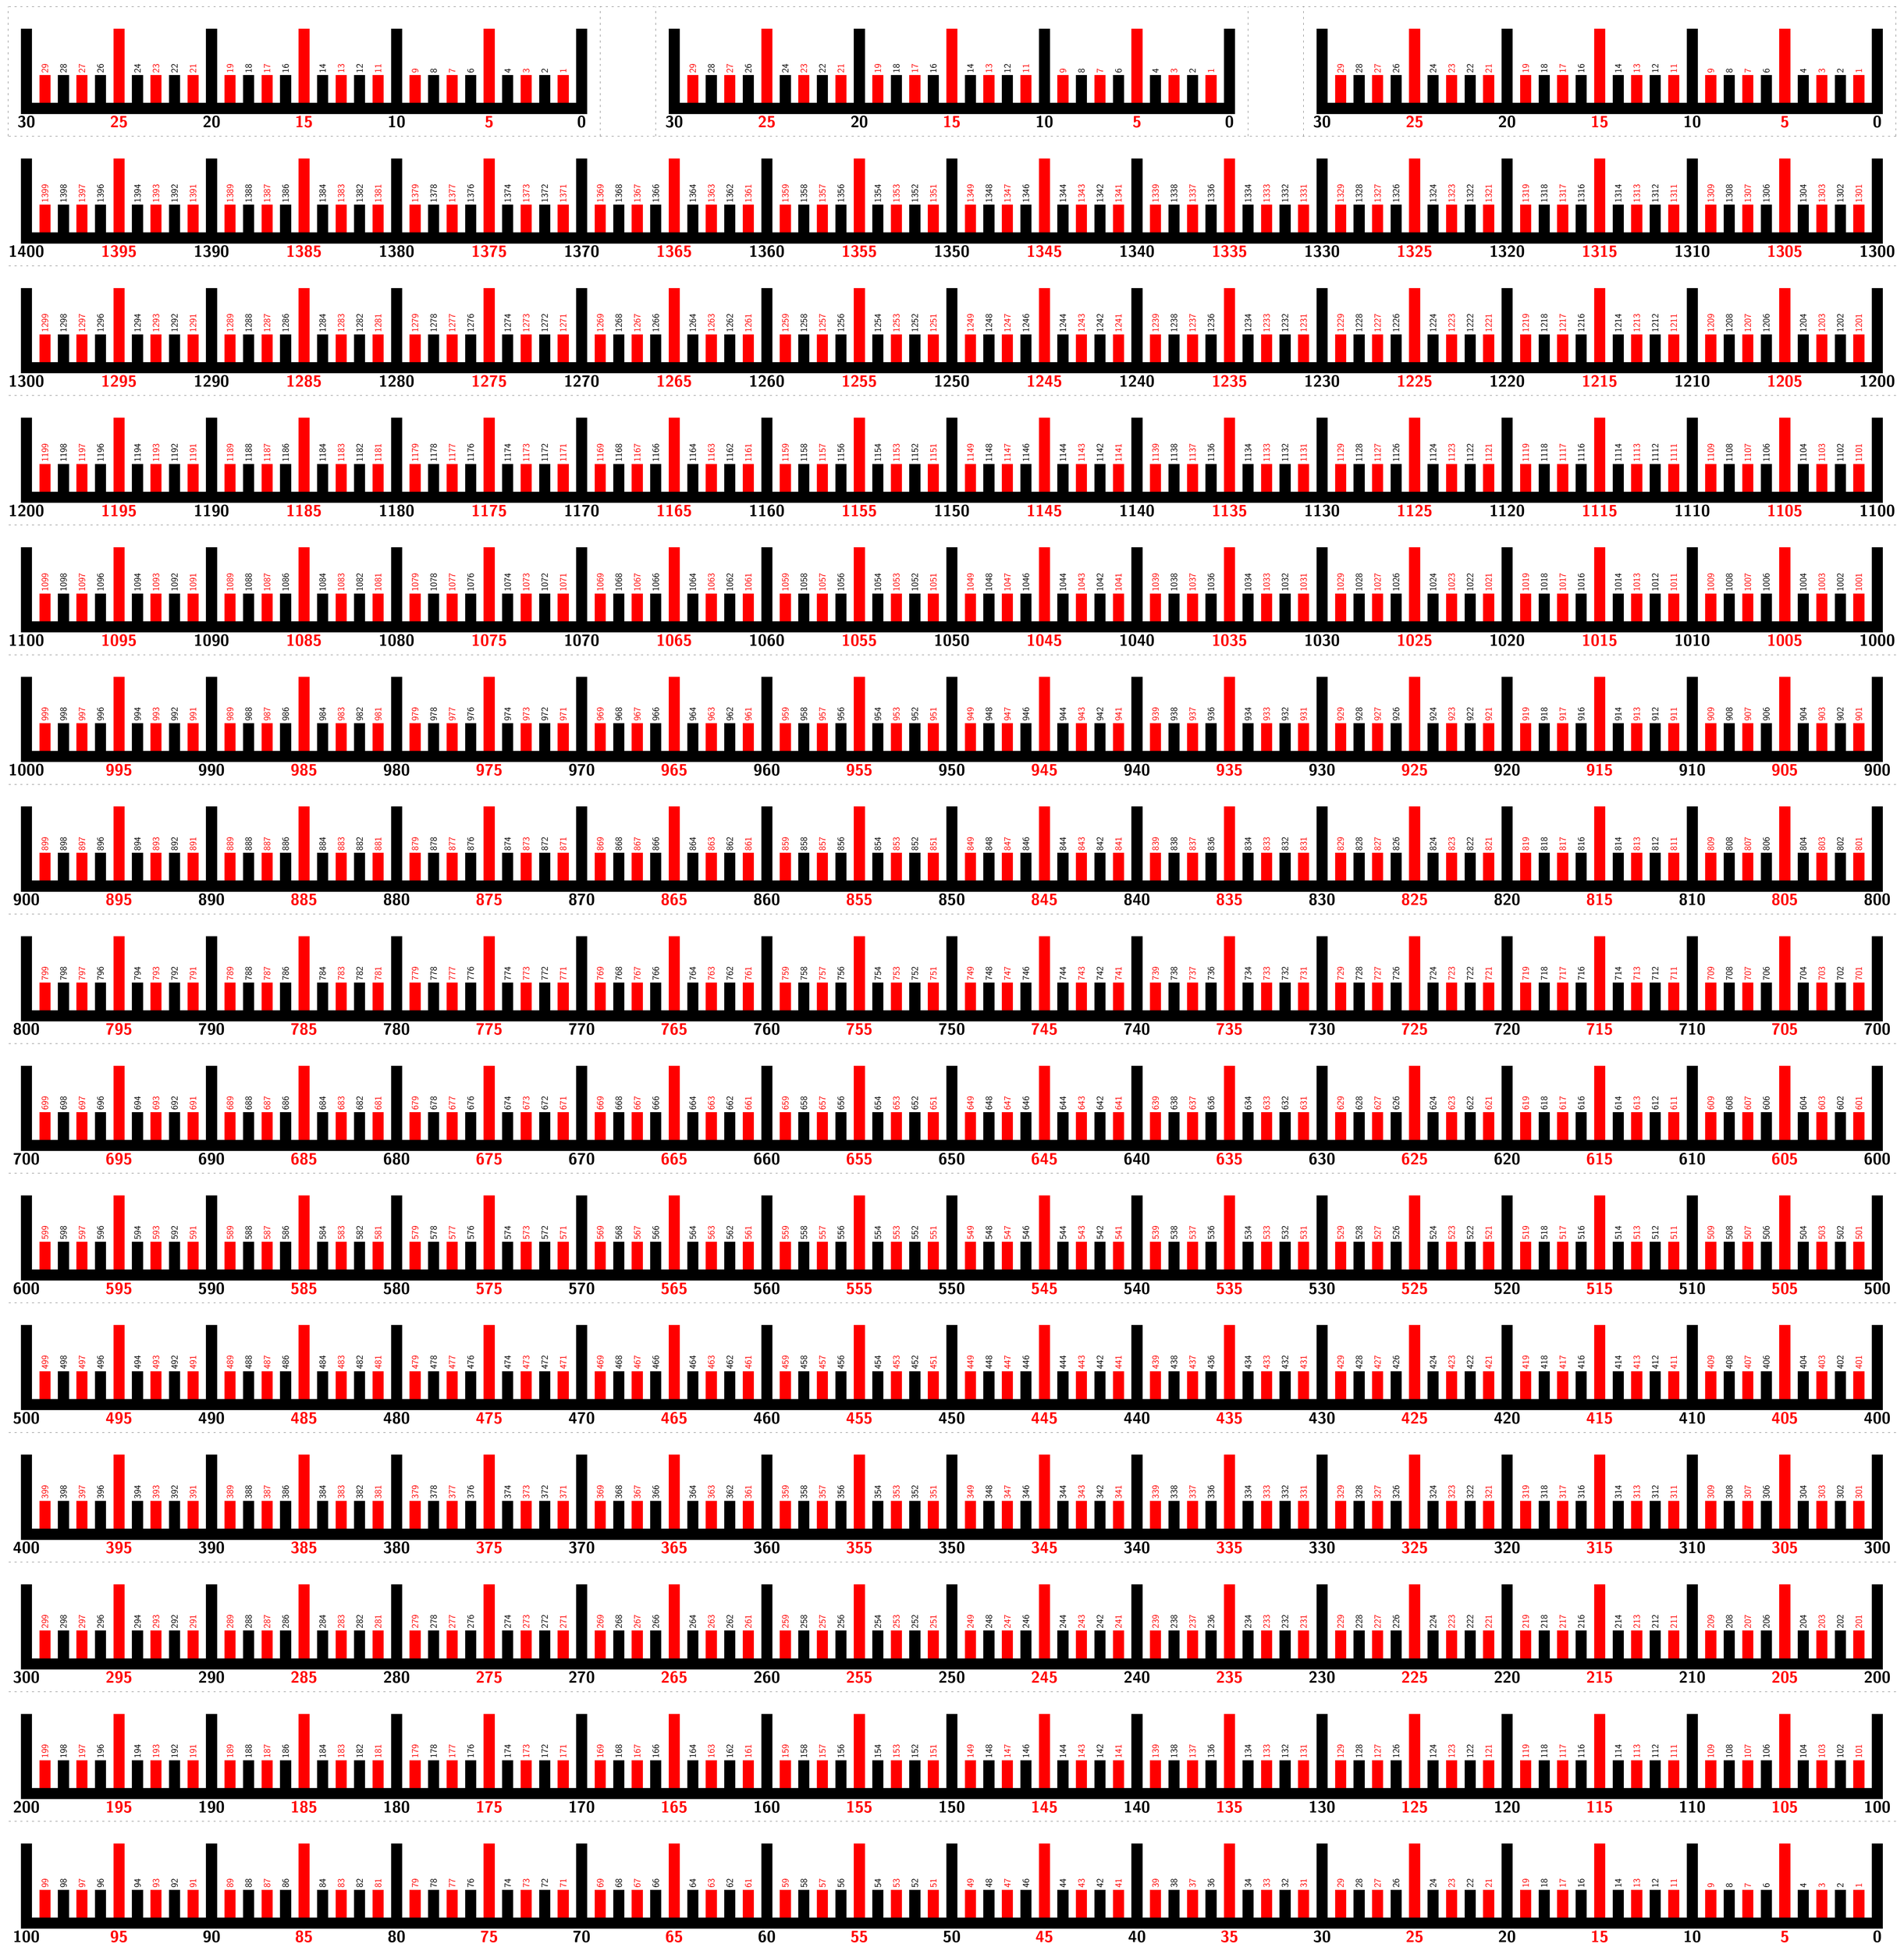
\begin{tikzpicture}[x=-1cm,line cap=rect]

  
  %%%% We need 3 x 14 rulers and each ruler will be offset 7 cm from the
  %%%% previous one. The commented out command allowed for the expansion of the
  %%%% \i %%%% variable and immediate concatenation with the 0. e.g., when \i =
  %%%% 3, %%%% yshift = \i0cm = 30cm.
  \foreach \i in {0,...,13}{
    % \tikzset{yshift/.expanded=\i0cm}
    \tikzset{yshift/.expanded=\i*7cm}
    

    %%%% Draw the red minor tick marks with the red labels. 
    \foreach \x in {1,3,...,99}
    \draw [color=red, line width=6mm](\x,0cm) -- (\x,1.5cm) 
    node[color=red, rotate=90, anchor=west] {\Large \pgfmathprint{int(\x+\i*100)}};   

    %%%% Draw the black minor tick marks with the black labels. 
    \foreach \x in {0,2,...,98}
    \draw [color=black, line width=6mm](\x,0cm) -- (\x,1.5cm) 
    node[color=black, rotate=90, anchor=west] {\Large \pgfmathprint{int(\x+\i*100)}};
    
    %%%% Draw the black major tick marks with the black labels. This paints over
    %%%% the minor tick marks in the same place.
    \foreach \x in {0,10,...,100}
    \draw [color=black,line width=6mm] (\x,4cm) -- (\x,0cm)
    node[anchor=north] {\Huge \textbf{{\pgfmathprint{int(\x+\i*100)}}}};

    %%%% Draw the red major tick marks with the red labels. This paints over
    %%%% the minor tick marks in the same place.
    \foreach \x in {5,15,...,95}
    \draw [color=red, line width=6mm] (\x,4cm) -- (\x,0cm)
    node[anchor=north] {\Huge \textbf{\pgfmathprint{int(\x+\i*100)}}};

    %%%% Draw the horizontal line that ties it all together.     
    \draw [line width=6mm](0, 0cm) -- coordinate (x axis mid) (100,0cm);

    %%%% Draw crop marks.
    \draw [very thin, color=black, loosely dashed](-1, 5.5cm) -- coordinate
    (x axis mid) (101,5.5cm);

    %%%% Capture the \i vertical coordinate
%    \xdef\lasti{\i}
  } 


  %%%% We also need 9 30-cm rulers. We will include three in this drawing. When
  %%%% everything is printed three times, we will have what we need. Yay! The
  %%%% vertical coordinate is hardcoded because I couldn't figure out how to
  %%%% propertly modify it after capturing the \i counter. 

  \foreach \j in {0,...,2}{
    % \tikzset{yshift/.expanded=\i0cm}
    \tikzset{xshift/.expanded=\j*-35cm}

    %%%% Draw the red minor tick marks with the red labels. 

    \foreach \x in {1,3,...,29}
    \draw [color=red, line width=6mm](\x,98cm) -- (\x, 99.5cm) 
    node[color=red, rotate=90, anchor=west] {\Large \pgfmathprint{int(\x)}}; 
    

    %%%% Draw the black minor tick marks with the black labels. 
    \foreach \x in {0,2,...,28}
    \draw [color=black, line width=6mm](\x, 98cm) -- (\x, 99.5cm) 
    node[color=black, rotate=90, anchor=west] {\Large \pgfmathprint{int(\x)}};
    
    %%%% Draw the black major tick marks with the black labels. This paints over
    %%%% the minor tick marks in the same place.
    \foreach \x in {0,10,...,30}
    \draw [color=black,line width=6mm] (\x, 102cm) -- (\x, 98cm)
    node[anchor=north] {\Huge \textbf{{\pgfmathprint{int(\x)}}}};

    %%%% Draw the red major tick marks with the red labels. This paints over
    %%%% the minor tick marks in the same place.
    \foreach \x in {5,15,...,25}
    \draw [color=red, line width=6mm] (\x,102cm) -- (\x,98cm)
    node[anchor=north] {\Huge \textbf{\pgfmathprint{int(\x)}}};

    %%%% Draw the horizontal line that ties it all together.     
    \draw [line width=6mm](0, 98 cm) -- coordinate (x axis mid) (30,98 cm);

    %%%% Draw vertical crop marks.
    \draw [very thin, color=black, loosely dashed](-1, 96.5cm) -- coordinate
    (x axis mid) (-1,103.5cm);
    
    \draw [very thin, color=black, loosely dashed](31, 96.5cm) -- coordinate
    (x axis mid) (31,103.5cm);


  }
    %%%% Draw crop marks.
    \draw [very thin, color=black, loosely dashed](-1, 103.5cm) -- coordinate
    (x axis mid) (101,103.5cm);

\end{tikzpicture}

\end{document}

%%% Local Variables: 
%%% mode: latex
%%% TeX-master: t
%%% End: 
